\documentclass[presentation.tex]{subfiles}

\begin{document}
\section{Mappings}
\begin{itemize}
    \item Mappings and corresponding patches are provided by the \href{https://inria.hal.science/hal-01948060/document}{Tokamesh}
            library (see Fig.~\ref{fig:tokamesh_grid}).
    \item Tokamesh uses the flux function from a Grad-Shafranov solver to construct mappings and 
            fit the patches accordingly to get flux aligned grids.
    \item $C^1$-conformity everywhere except close to the X-point.
\end{itemize}
\begin{figure}
    \centering
    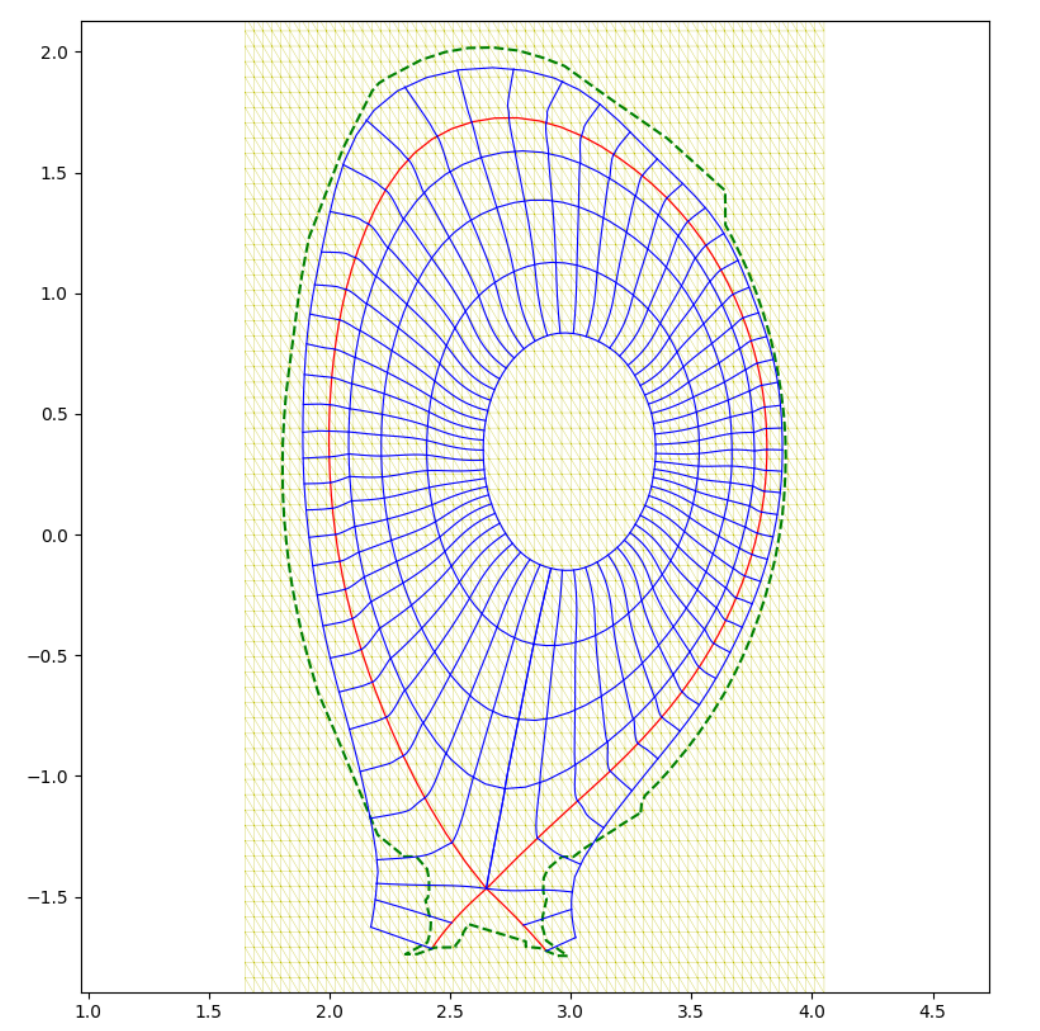
\includegraphics[width=0.8 \textwidth]{images/tokamesh_grid.png}
    \caption{Flux-aligned multipatch grid (blue lines) 
             from \href{https://inria.hal.science/hal-01948060/document}{Tokamesh}}
    \label{fig:tokamesh_grid}
\end{figure}
\end{document}